\documentclass[review,onecolumn]{vgtc}                % final (journal style)
%\documentclass[11pt,onecolumn,review,journal]{vgtc}         % review (journal style)
%\documentclass[widereview]{vgtc}             % wide-spaced review
%\documentclass[preprint,journal]{vgtc}       % preprint (journal style)
%\documentclass[electronic,journal]{vgtc}     % electronic version, journal

%% Uncomment one of the lines above depending on where your paper is
%% in the conference process. ``review'' and ``widereview'' are for review
%% submission, ``preprint'' is for pre-publication, and the final version
%% doesn't use a specific qualifier. Further, ``electronic'' includes
%% hyperreferences for more convenient online viewing.

%% Please use one of the ``review'' options in combination with the
%% assigned online id (see below) ONLY if your paper uses a double blind
%% review process. Some conferences, like IEEE Vis and InfoVis, have NOT
%% in the past.

%% Please note that the use of figures other than the optional teaser is not permitted on the first page
%% of the journal version.  Figures should begin on the second page and be
%% in CMYK or Grey scale format, otherwise, colour shifting may occur
%% during the printing process.  Papers submitted with figures other than the optional teaser on the
%% first page will be refused.

%% These three lines bring in essential packages: ``mathptmx'' for Type 1
%% typefaces, ``graphicx'' for inclusion of EPS figures. and ``times''
%% for proper handling of the times font family.

\usepackage{mathptmx}
\usepackage{graphicx}
\usepackage{times}

\usepackage{wrapfig}
\usepackage{amsmath,amssymb}
\usepackage{setspace}
\usepackage{color, colortbl}
\usepackage{pdfpages}
\usepackage{booktabs}
%\usepackage{CJK}

\usepackage{algorithm}
\usepackage{algorithmicx}
\usepackage{algpseudocode}
\usepackage{geometry}

\geometry{a4paper}


\usepackage{anyfontsize}
\usepackage{textcomp}


% *** SUBFIGURE PACKAGES ***

\usepackage{url}

\graphicspath{{../figures/}} % where to search for the images
% *** SUBFIGURE PACKAGES ***
%

\usepackage[caption=false,font=footnotesize]{subfig}

%\usepackeage{colors}
\usepackage{caption}
\renewcommand{\vec}[1]{\mathbf{#1}}
\renewcommand{\d}{\textrm{d}}
%\usepackage[font=sf, labelfont={sf,bf}, margin=1cm]{caption}
\usepackage[shortlabels]{enumitem}
\include{macros}
\definecolor{gray}{rgb}{0.65,0.65,0.65}
\definecolor{green}{rgb}{0, 0.5, 0}
\definecolor{orange}{rgb}{0.8, 0.6, 0.2}
\definecolor{red}{rgb}{1.0, 0.0, 0.0}
\definecolor{teal}{rgb}{0.0, 0.4, 0.4}
\definecolor{purple}{rgb}{0.65,0,0.65}
\definecolor{pink}{rgb}{1.0,0.1,0.6}
\definecolor{blue}{rgb}{0.0,0.1,1.0}

\newcommand{\Rspace}{\mathbb{R}}
\newcommand{\Mspace}{\mathbb{M}}
\newcommand{\T}{\mathbb{T}}
\providecommand{\shortcite}[1]{\cite{#1}}
\newenvironment{my_enumerate}{
\begin{enumerate}
  \setlength{\itemsep}{1pt}
  \setlength{\parskip}{0pt}
  \setlength{\parsep}{0pt}}{\end{enumerate}
}

\newenvironment{my_itemize}{
\begin{itemize}
  \setlength{\itemsep}{1pt}
  \setlength{\parskip}{0pt}
  \setlength{\parsep}{0pt}}{\end{itemize}
}

\newcommand{\myparagraph}[1]{\mbox{\ } \newline \noindent \textbf{#1}}
\renewcommand{\paragraph}[1]{\myparagraph{#1}}

\usepackage{enumitem}
\usepackage{pdfpages}
\usepackage{multirow}

\newcommand{\yh}[1]{{\color{orange}[yunhai: #1]}}
\newcommand{\od}[1]{{\color{red}[OD: #1]}}
\newcommand{\phil}[1]{{\color{green}[ph: #1]}}

\newcommand{\toolname}{$\mathbb{C}^3$}



\newcommand{\new}[1]{{\color{blue}#1}}


\DeclareMathOperator*{\argmin}{\arg\,min}

%% We encourage the use of mathptmx for consistent usage of times font
%% throughout the proceedings. However, if you encounter conflicts
%% with other math-related packages, you may want to disable it.

%% This turns references into clickable hyperlinks.
\usepackage[bookmarks,backref=true,linkcolor=black]{hyperref} %,colorlinks
\hypersetup{
  pdfauthor = {},
  pdftitle = {},
  pdfsubject = {},
  pdfkeywords = {},
  colorlinks=true,
  linkcolor= black,
  citecolor= black,
  pageanchor=true,
  urlcolor = black,
  plainpages = false,
  linktocpage
}


% Hide or show our comments
\newif\ifshowcomments
\showcommentstrue
%\showcommentsfalse

% Coloring for our comments (use showcommentstrue or showcommentsfalse above to show/hide)


%% If you are submitting a paper to a conference for review with a double
%% blind reviewing process, please replace the value ``0'' below with your
%% OnlineID. Otherwise, you may safely leave it at ``0''.

%\onlineid{1213}

\onlineid{4276}

\title{\toolname-palette: Co-saliency based Colorization for Comparing Categorical Visualizations \\
[1ex]\begin{LARGE} -- Supplementary Material -- \end{LARGE}}

%% Uncomment below to disable the manuscript note
%\renewcommand{\manuscriptnotetxt}{}

%% Copyright space is enabled by default as required by guidelines.
%% It is disabled by the 'review' option or via the following command:
% \nocopyrightspace

%%%%%%%%%%%%%%%%%%%%%%%%%%%%%%%%%%%%%%%%%%%%%%%%%%%%%%%%%%%%%%%%
%%%%%%%%%%%%%%%%%%%%%% START OF THE PAPER %%%%%%%%%%%%%%%%%%%%%%
%%%%%%%%%%%%%%%%%%%%%%%%%%%%%%%%%%%%%%%%%%%%%%%%%%%%%%%%%%%%%%%%%

\begin{document}

\newcounter{partextdummy}
\newcommand*{\CreateLink}[2]{%
  \begingroup
    \renewcommand*{\thepartextdummy}{#2}%
    \ifhmode
      % raise the anchor above the base line in horizontal mode
      \raisebox{2ex}[0pt][0pt]{%
        \refstepcounter{partextdummy}%
        \label{#1}%
      }%
    \else
      \refstepcounter{partextdummy}%
      \label{#1}%
    \fi
  \endgroup
  \ignorespaces
}
\newcommand*{\LinkTo}{\ref}

%% The ``\maketitle'' command must be the first com\cite{}mand after the
%% ``\begin{document}'' command. It prepares and prints the title block.

%% the only exception to this rule is the \firstsection command
\maketitle

This supplementary material provides additional experimental results for our submitted paper titled ``\toolname-palette: Co-saliency based Colorization for Comparing Categorical Visualizations''.
%
%\paragraph{Overview}\\
%We include materials for:
%
%\vspace{-2mm}
%\begin{enumerate}[start=1]
%\item \LinkTo{overlappedScatterplots}
%\vspace{-2mm}
%\item \LinkTo{badcaseAB}
%\vspace{-2mm}
%\item \LinkTo{pilotStudy}
%\vspace{-2mm}
%\item \LinkTo{caseStudy}
%\vspace{-2mm}
%\item \LinkTo{colorBlindness}
%\vspace{-2mm}
%\end{enumerate}

%%%%%%%%%%%%%%%%%%%%%%%%%%%%%%%%%%%%%%%%%%%%%%%%

\CreateLink{overlappedScatterplots}{Scatterplots with Significant Overlap}
\paragraph{Scatterplots with Significant Overlap}.
Since our contrast measures are built on data-space nearest neighbour graphs, their produced palettes also work well for scatterplots with significant overlap between classes. For example, as shown in the results from the \emph{Random Assignment} in Fig.~\ref{fig:scatterOverlap}, the light orange class is mixed with the light purple class and the teal class has a strong overlap with the grey class, all of them are hard to distinguish. The \emph{Alpha Blending} result is based on \emph{Optimized Assignment}~\cite{Wang2018} with the Tableau palette; however, due to the changed opacity, classes are hard to split from each other and new colors appear. The results generated from \emph{Palettailor} and \emph{$C^3$-palette} have a good separability since both are built on data-space nearest neighbour graphs. Specifically, \emph{$C^3$-palette} highlights  changed classes (classes with green, purple and red) while maintaining discrimination of strong overlapped classes, such as the blue and yellow, red and green classes.

\begin{figure}[h]
\centering
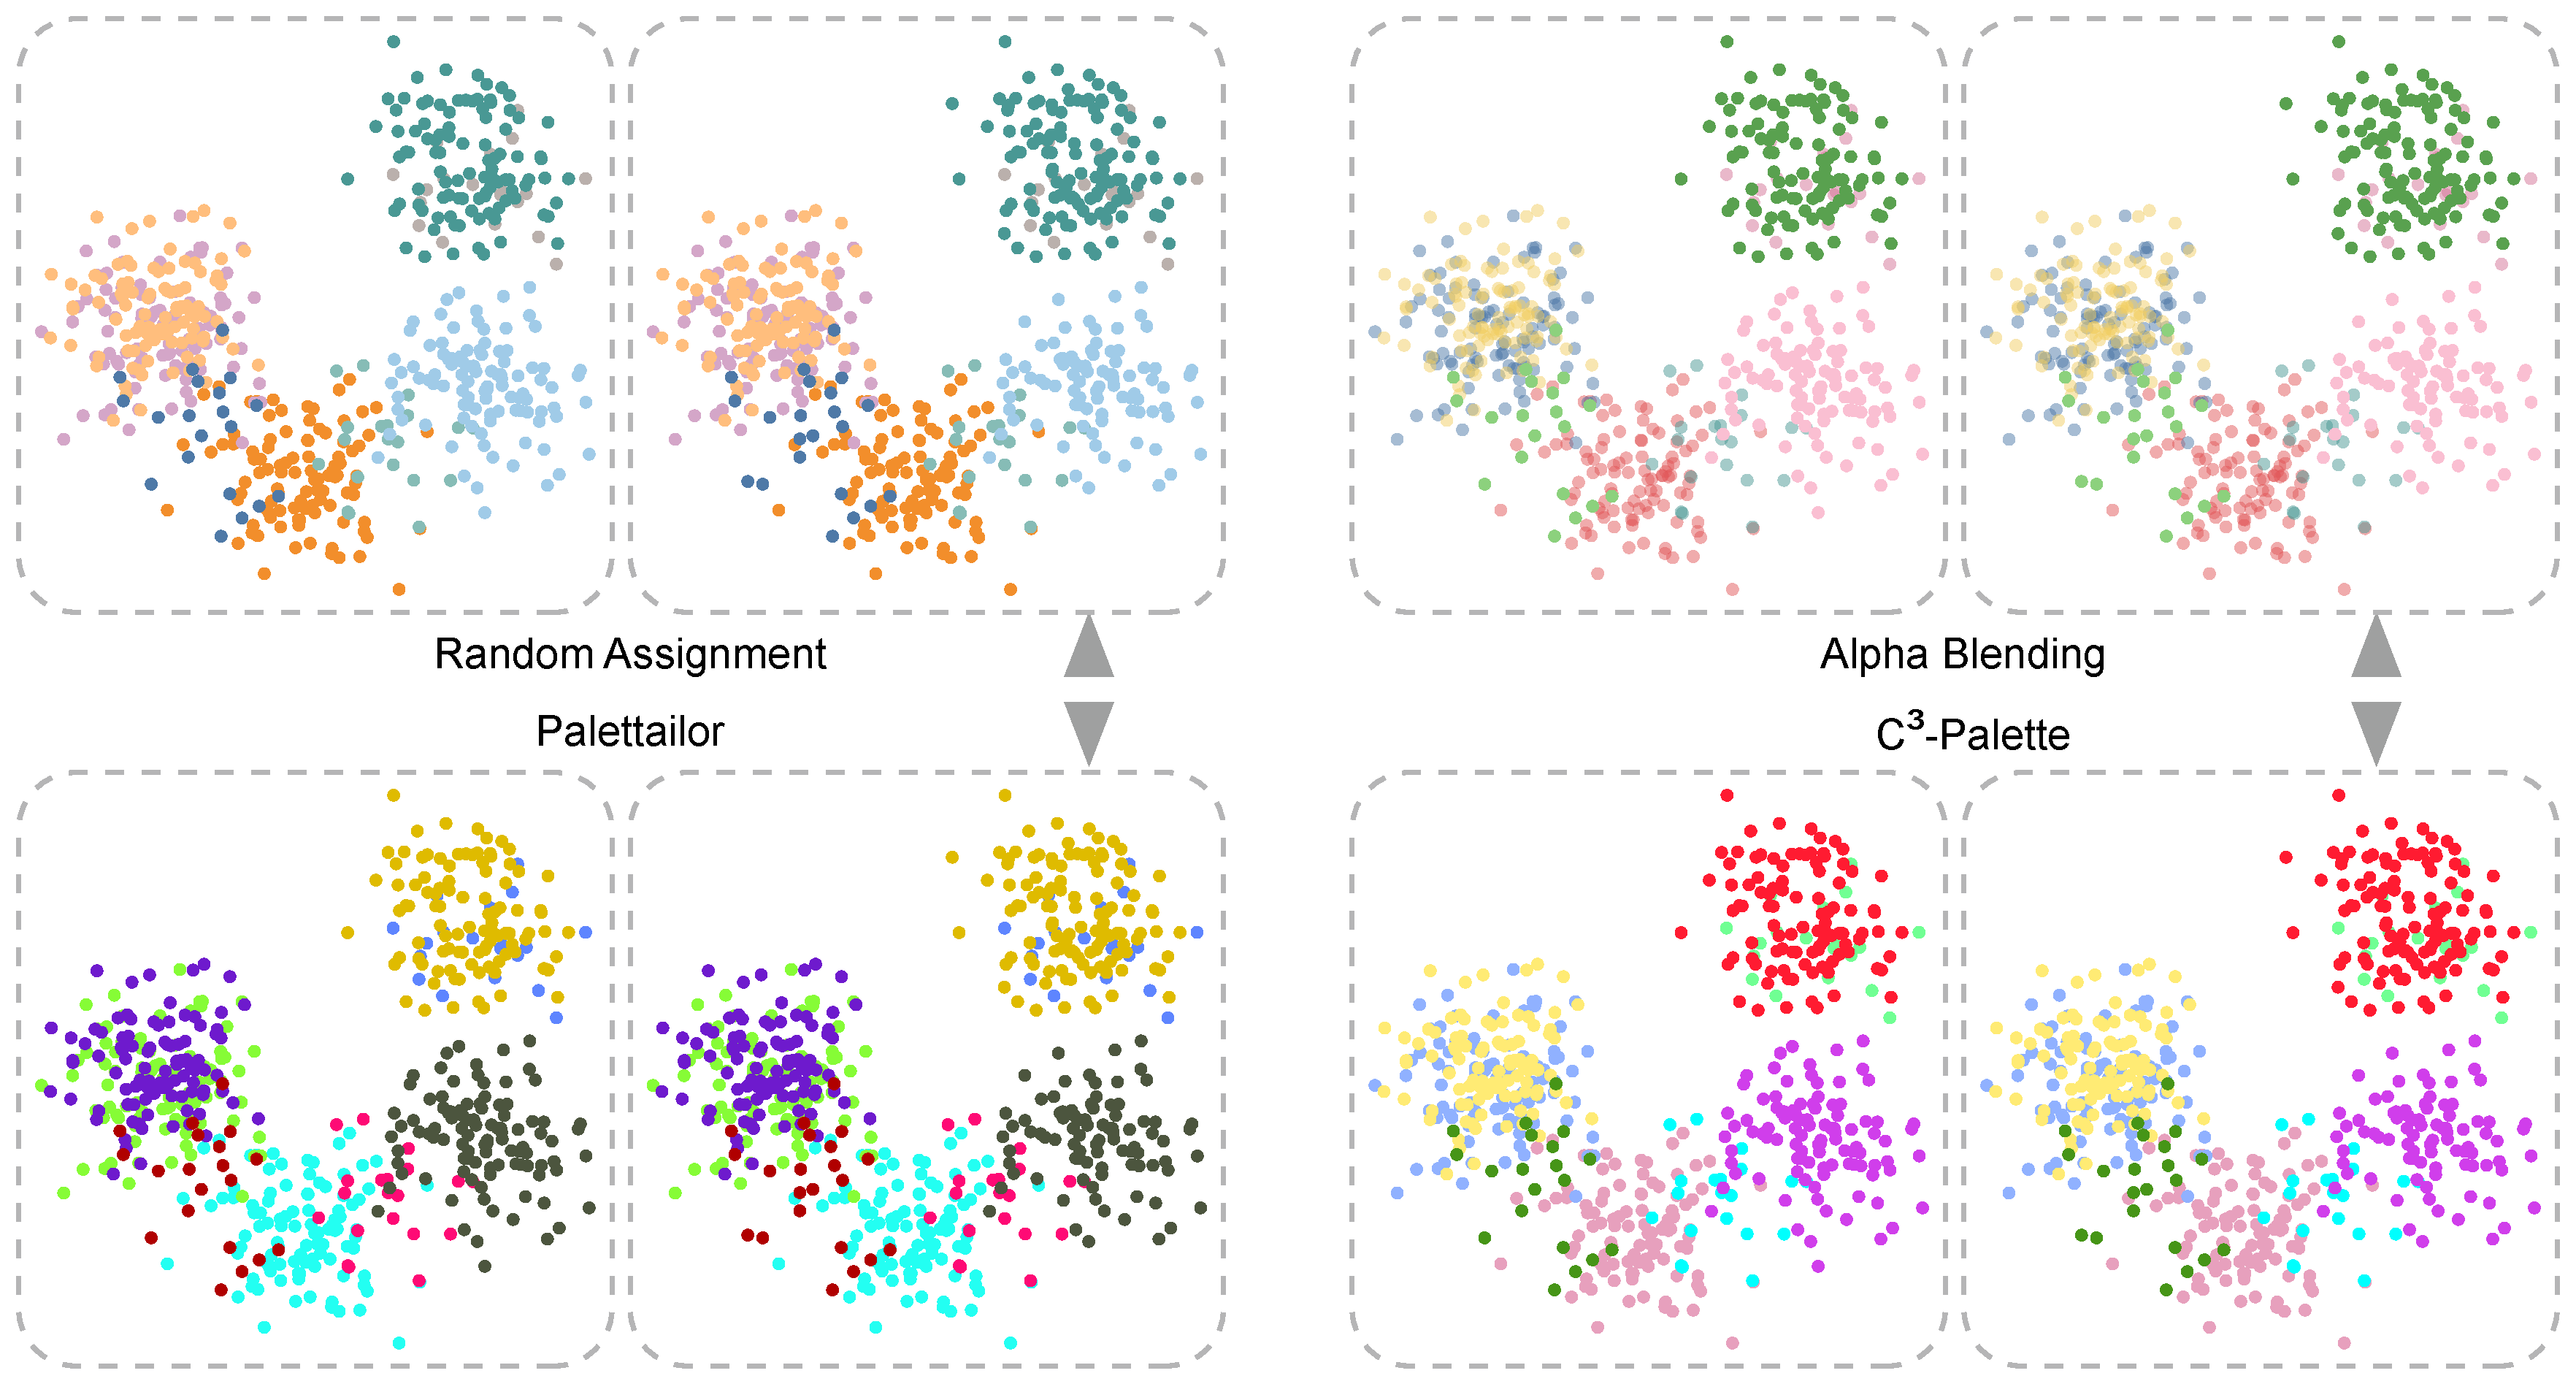
\includegraphics[width=1\linewidth]{scatter-overlap.pdf}
\caption{Results for scatterplots with significant overlap: (left) Tableau palette with random assignment versus Palettailor~\cite{Lu21}; (right) Alpha Blending versus $C^3$-palette. Our co-saliency methods (right bottom) are able to highlight changed classes while maintaining discrimination of strongly overlapping classes.}
\vspace*{-3mm}
\label{fig:scatterOverlap}
\end{figure}

\CreateLink{badcaseAB}{Bad Case for Alpha Blending on Different Visualizations}
\paragraph{Bad Cases for Alpha Blending on Different Visualizations}.
In the previous section, we show that overlapping scatterplot points would composite new colors in the case of alpha blending. Here we show that alpha blending is insufficient even for bar and line charts. Fig.~\ref{fig:badcaseAB} shows an example, where the two images on the top left show our auto-generated results, on the bottom left are  alpha blending results based on the Tableau 20 palette. We maintained an opacity of 1.0 for the bar with the largest difference, while changing the opacity of the others to 0.4. It is still hard to find the largest change immediately. This effect also exists in the line chart shown in Fig.~\ref{fig:badcaseAB} right. Due to the low contrast against the background, the yellow line does not pop out visually even when the opacity of the other classes set to 0.2.

\begin{figure}[ht]
\centering
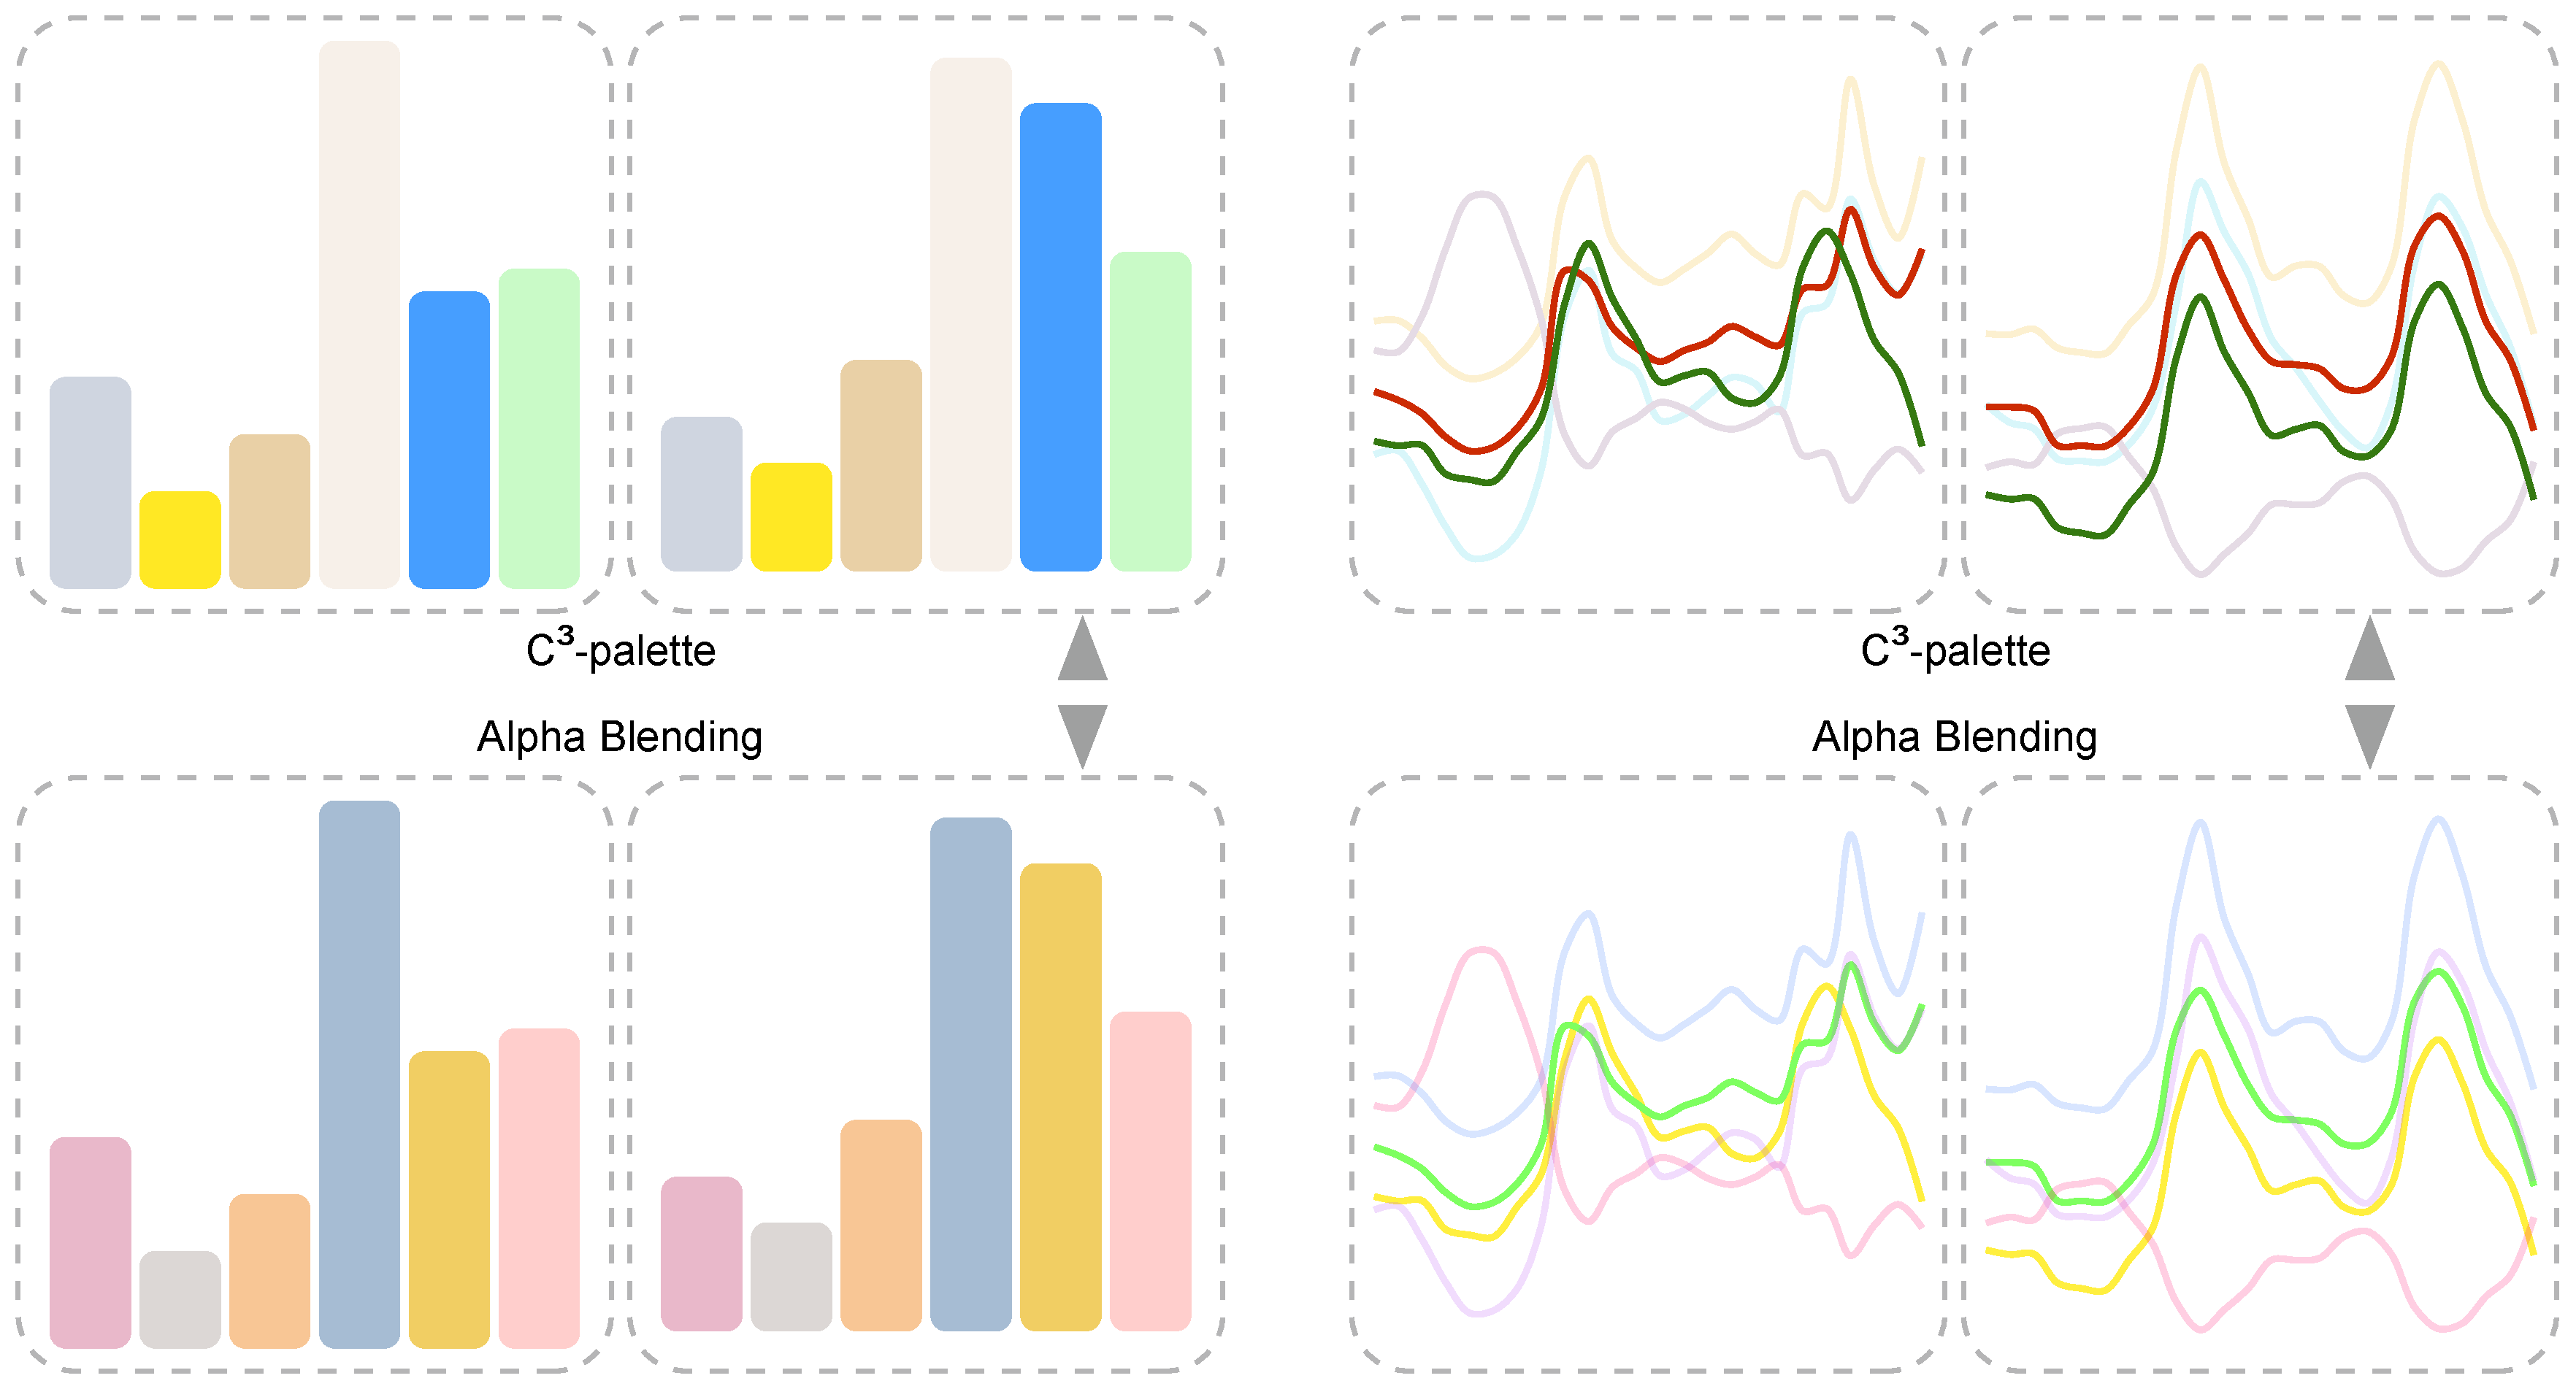
\includegraphics[width=0.96\linewidth]{badcaseAB.pdf}
\caption{The problem of alpha blending: (left) $C^3$-palette versus Tableau palette with alpha blending for bar charts; (right) $C^3$-palette versus a palette with low contrast colors using alpha blending for line charts.}
\vspace*{-5mm}
\label{fig:badcaseAB}
\end{figure}


\CreateLink{pilotStudy}{Pilot Study Details and Statistics}
\paragraph{Pilot Study Details and Statistics}.
We conducted two pilot studies for the scatterplot experiment, one \emph{identifying delta task} and a \emph{counting class task}. The statistical results are shown in Fig.~\ref{fig:pilotResults}.
For the \emph{identifying delta task}, we recruited $28$ people (see Table.~\ref{tab:participantDetail}) through Amazon Mechanical Turk. The power analysis was computed between \emph{$C^3$-palette Generation} and \emph{Random Assignment}. With an effect size Cohen's $d$ of $0.4$, an alpha level of $0.05$ and a beta level of $0.8$, the power analysis suggested a minimum number of $100$ participants for this task.
The procedure of \emph{counting class task} was similar to the previous one. We recruited 29 participants from AMT whose approval rate was larger than $97\%$. Since we mainly wanted to compare the class discriminability between \emph{$C^3$-palette Generation} and \emph{Alpha Blending}, we executed the power analysis based on these two conditions.  With an effect size Cohen's $d$ of $0.6$, the analysis indicated that we needed 50 participants for this task.

\begin{figure*}[h]
\centering
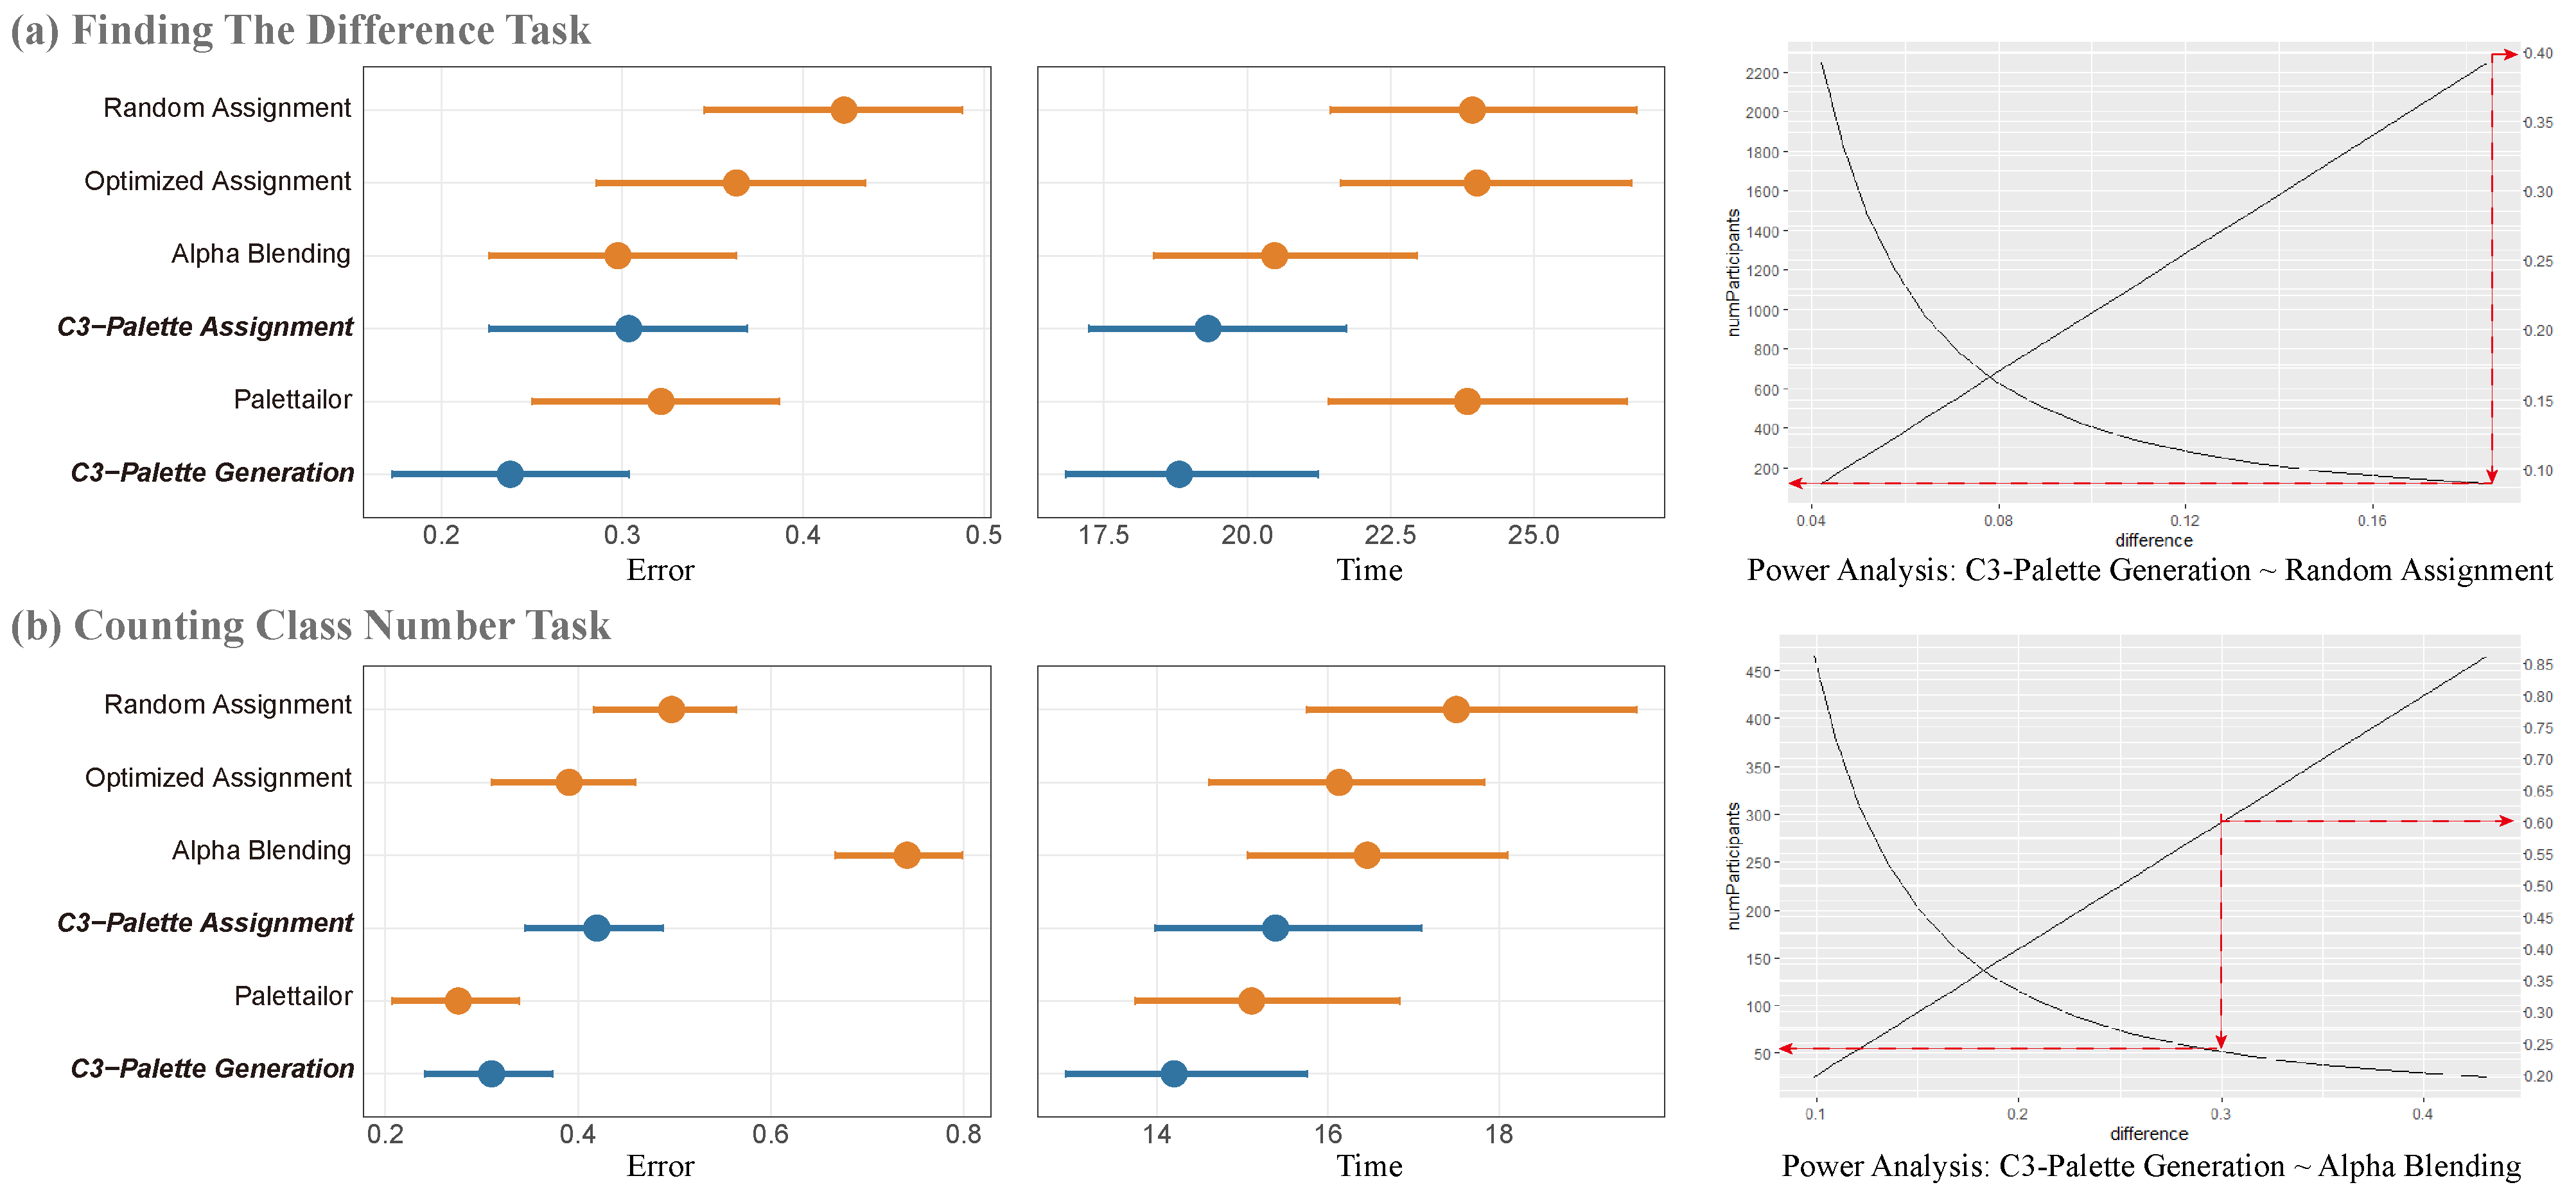
\includegraphics[width=1\linewidth]{user-result-pilot.pdf}
\caption{Confidence interval plots and power analysis for the two pilot studies.}
\vspace*{-5mm}
\label{fig:pilotResults}
\end{figure*}

\begin{table}[ht]
\renewcommand\arraystretch{1}
\centering
\caption{Participants details for each task within the scatterplot experiment.}
\label{tab:participantDetail}
\begin{tabular}{|c|c|c|c|c|}
\hline
\multirow{2}{*}{\textbf{Task \& Group}} & \multicolumn{2}{c|}{identifying delta task} & \multicolumn{2}{c|}{counting class task} \\
\cline{2-5}
& Pilot(28) & Formal(108) & Pilot(29) & formal(52) \\
\hline
Group 1 & 5 & 18 & 5  & 9 \\
\hline
Group 2 & 5 & 17 & 5  & 8 \\
\hline
Group 3 & 5 & 19 & 4  & 8 \\
\hline
Group 4 & 3 & 17 & 5  & 9 \\
\hline
Group 5 & 5 & 19 & 5  & 9 \\
\hline
Group 6 & 5 & 18 & 5  & 9 \\
\hline
\end{tabular}
\end{table}

\CreateLink{formalStudy}{Formal Study Statistics Results}
\paragraph{Formal Study Statistics Results}.
Here we show the detailed results. The statistics are shown in Fig.~\ref{fig:formalStudy}.

\begin{figure*}[h]
\centering
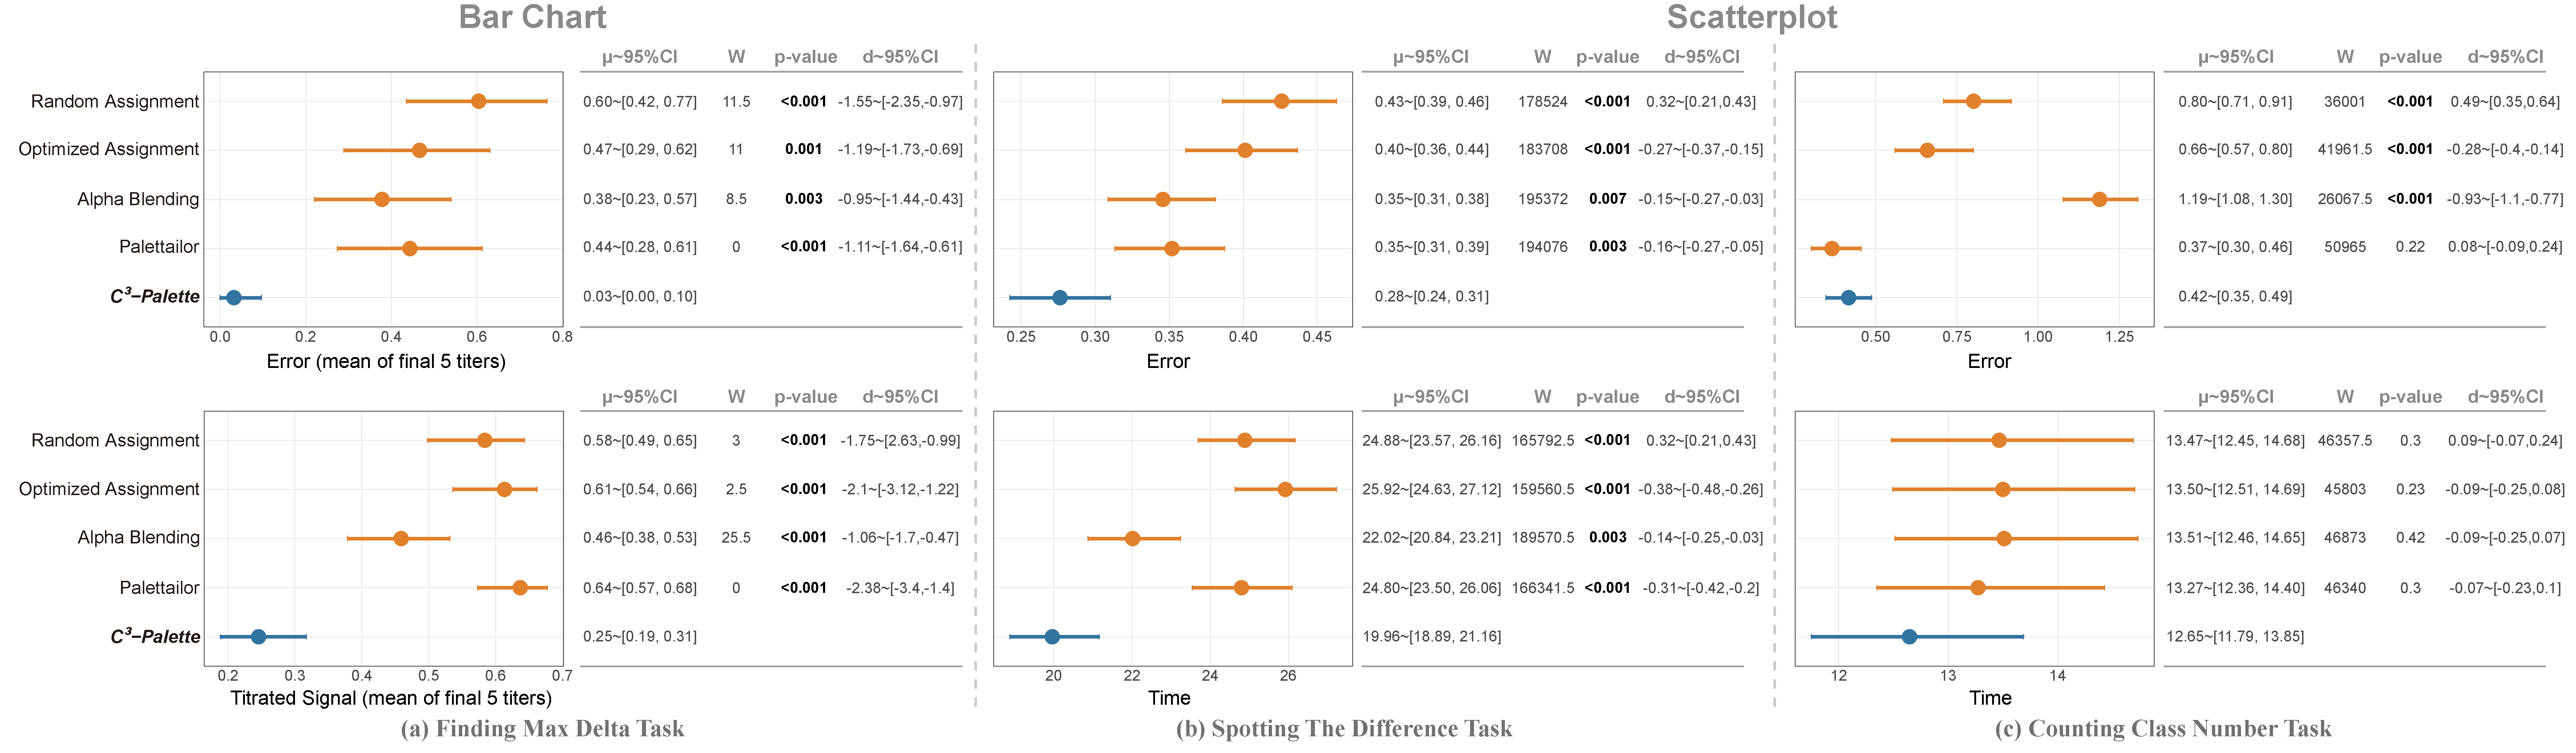
\includegraphics[width=1\linewidth]{formal-statistics-results.pdf}
\caption{Confidence intervals and statistical tables for the online controlled experiment. The error bars represent 95\% confidence intervals. Each table shows the test results for the  \emph{$C^3$-palette Generation} condition compared to the other conditions, including the mean with 95\% confidence interval ($\mu\sim$95\%CI), the W-value and p-value from the Mann-Whitney test, and the effect size ($d\sim$95\%CI).
}
\vspace*{-5mm}
\label{fig:formalStudy}
\end{figure*}

%
%\CreateLink{caseStudy}{Additional Case Study for Scatterplots}
%\paragraph{Additional Case Study for Scatterplots}.
%We conducted a case study with a real world data, which is well-known for the use in Gapminder~\cite{gapminder}, to evaluate the usability of our system.
%
%\begin{figure}[h]
%\centering
%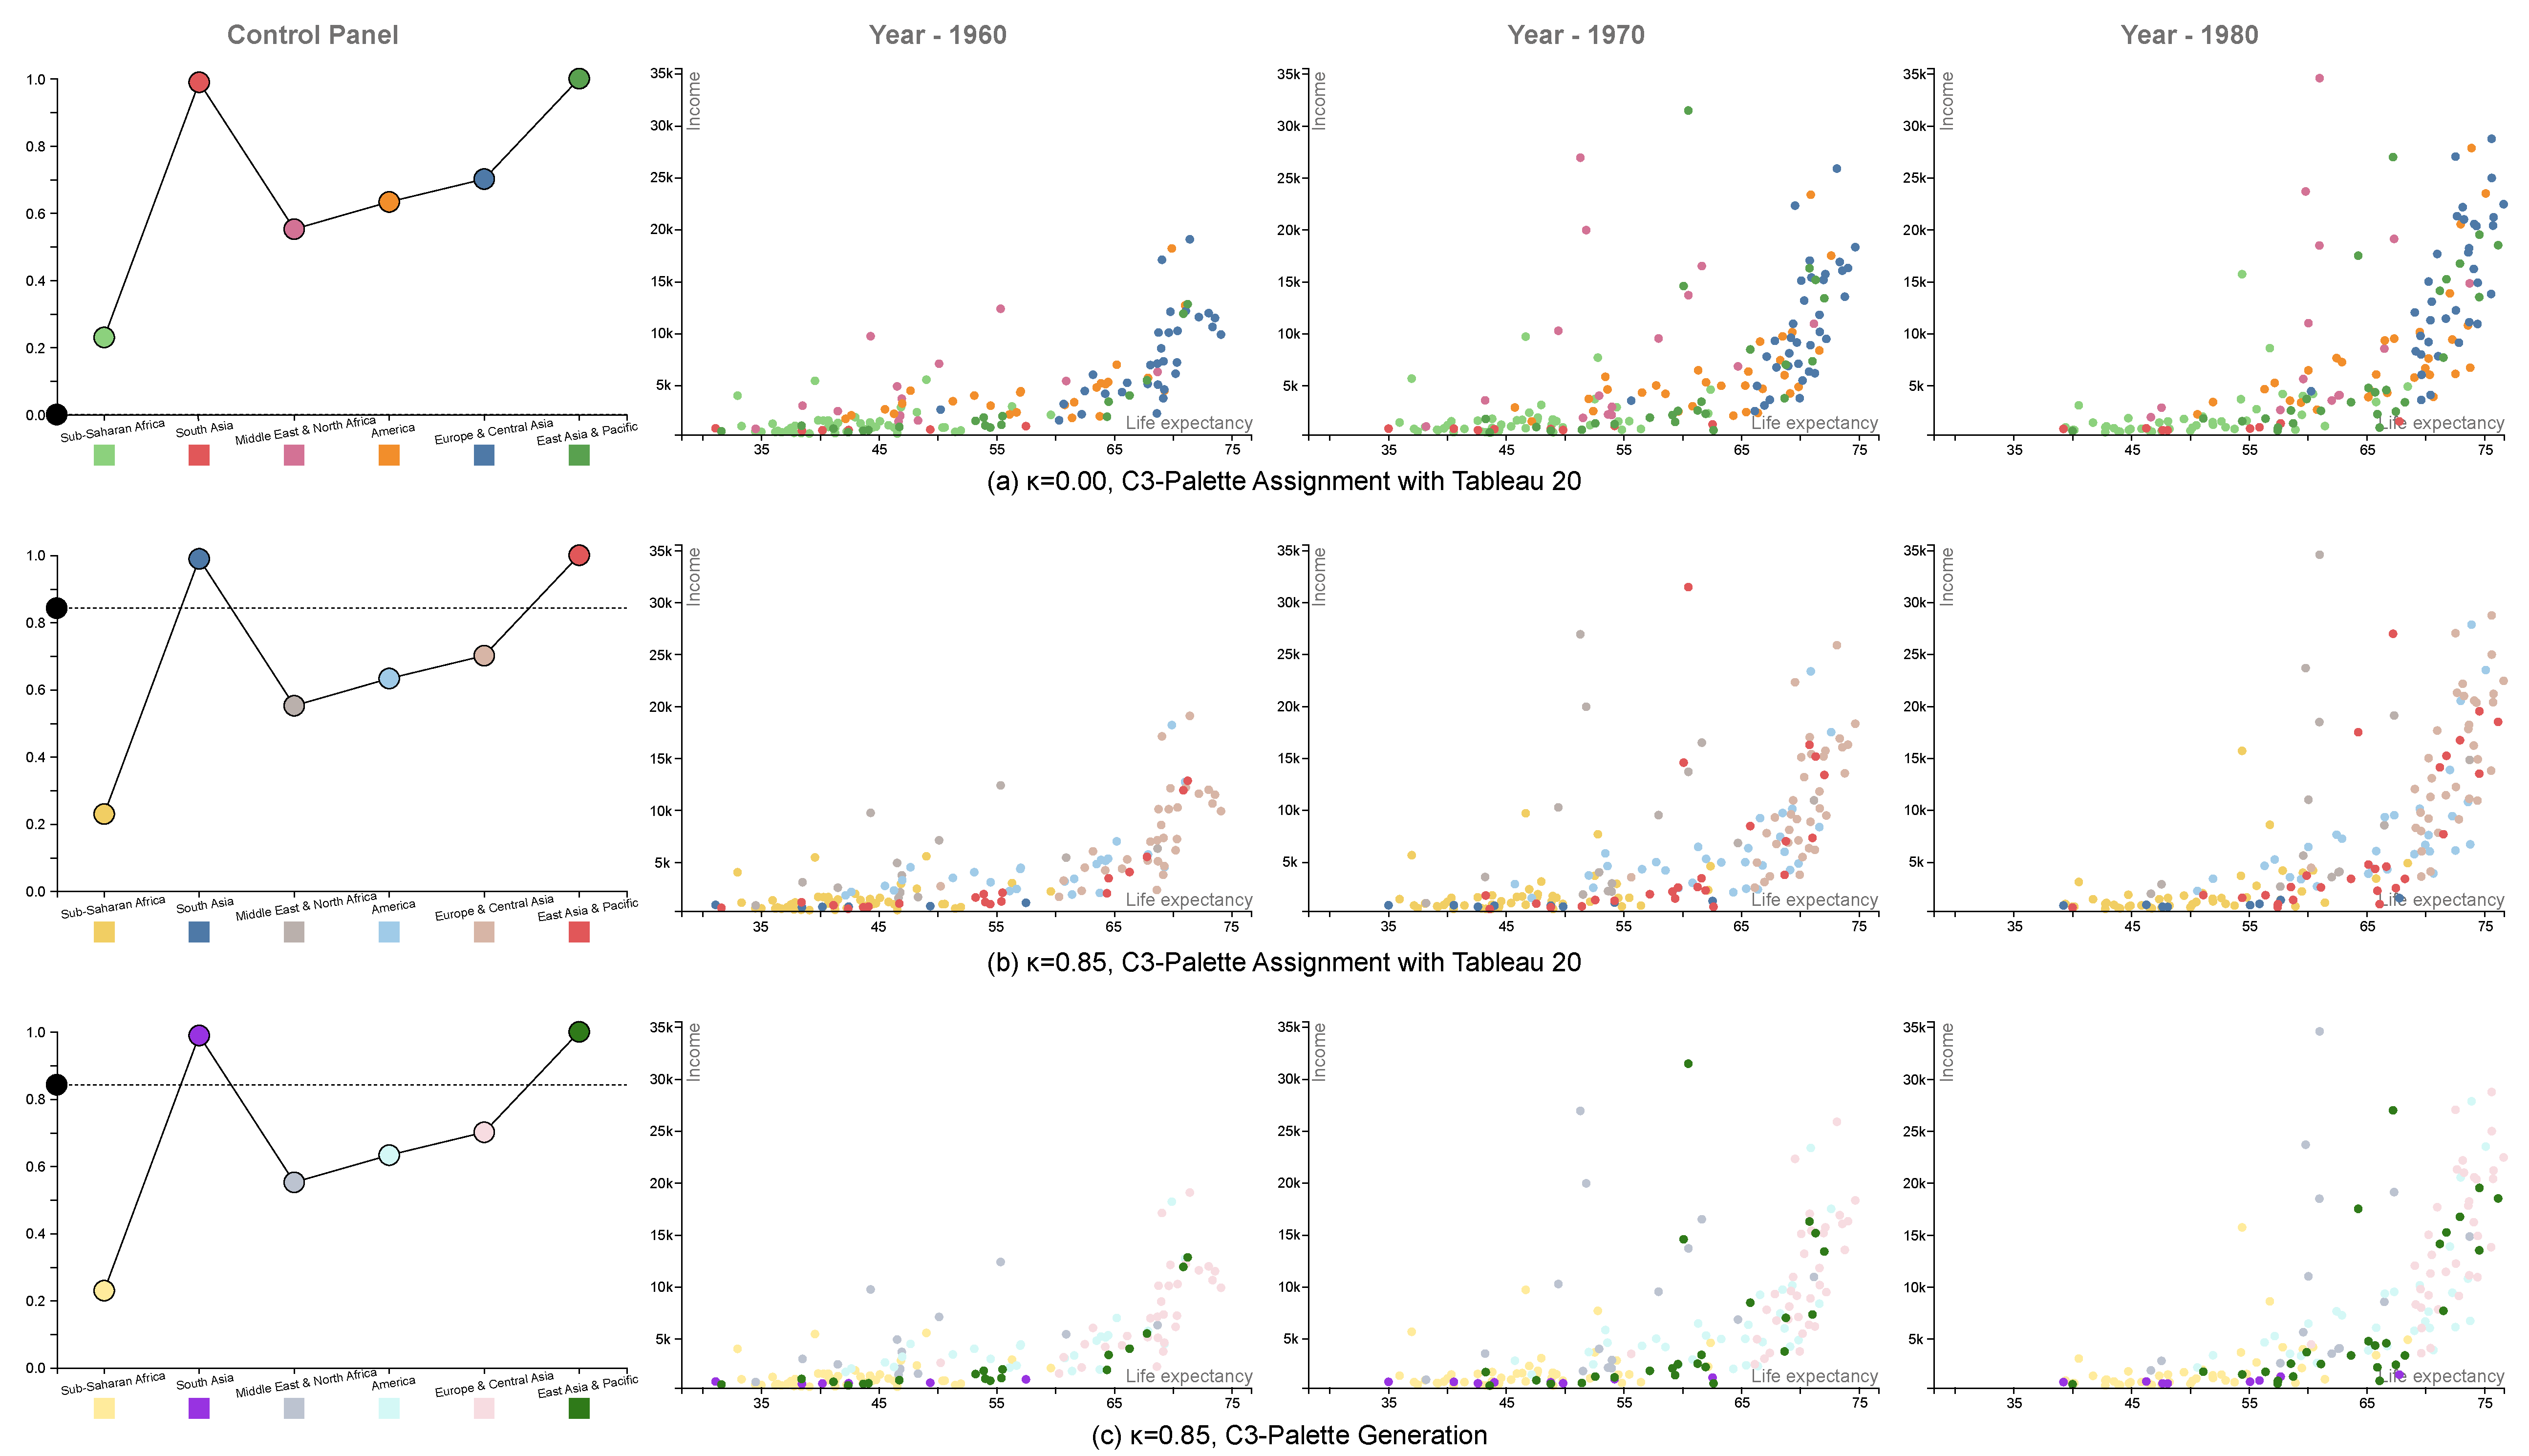
\includegraphics[width=\linewidth]{case-study.pdf}
%\caption{Gapminder dataset: (a) Result generated by default setting for given palette; (b) User-specified $\kappa$ value for popping out classes; (c) Automatic palette generation for achieving a better discriminablity.}
%\label{fig:casestudy}
%\vspace{-3mm}
%\end{figure}
%We choose life expectancy and income as the x axis and y axis, respectively. And we use world regions as the class label. As shown in Fig.~\ref{fig:casestudy}, due to the limit space, we only show three years. And to make it easy to read, we removed the points with a much larger x value or y value.
%First, we used the default settings of our system to automatically produce a color assignment result based on Tableau 20 palette for assigning colors to different objects in the dataset, see Fig.~\ref{fig:casestudy}(a). Since $\kappa$ is $0$ and all the classes are changed, each class is assigned with a salient color to make it more distinguishable. This result is similar to \emph{Optimized Assignment}~\cite{Wang2018} while our result considers the different importance of classes, i.e., larger importance value has a more salient color.
%Then we want to explore the two classes with the largest change degree, thus we move the $\kappa$ control point(the black circle in control panel) to a larger value, as shown in Fig.~\ref{fig:casestudy}(b). Now we can see the largest changed classes more clearly. But the visual separability between the classes with lower $\kappa$ value is small, such as the color of \emph{Middle East \& North Africa} and \emph{Europe \& Central Asia}. We further generate the result by our palette generation method which has a better performance on discriminability, see Fig.~\ref{fig:casestudy}(c).
%Through our exploration, we found that \emph{South Asia} should not have a large change degree. This result is caused by our default class importance measure which sets point number change a larger weight, this is done due to the previous evaluation result that point number change is harder to distinguish than point position change.
%
%\begin{figure}[h]
%\centering
%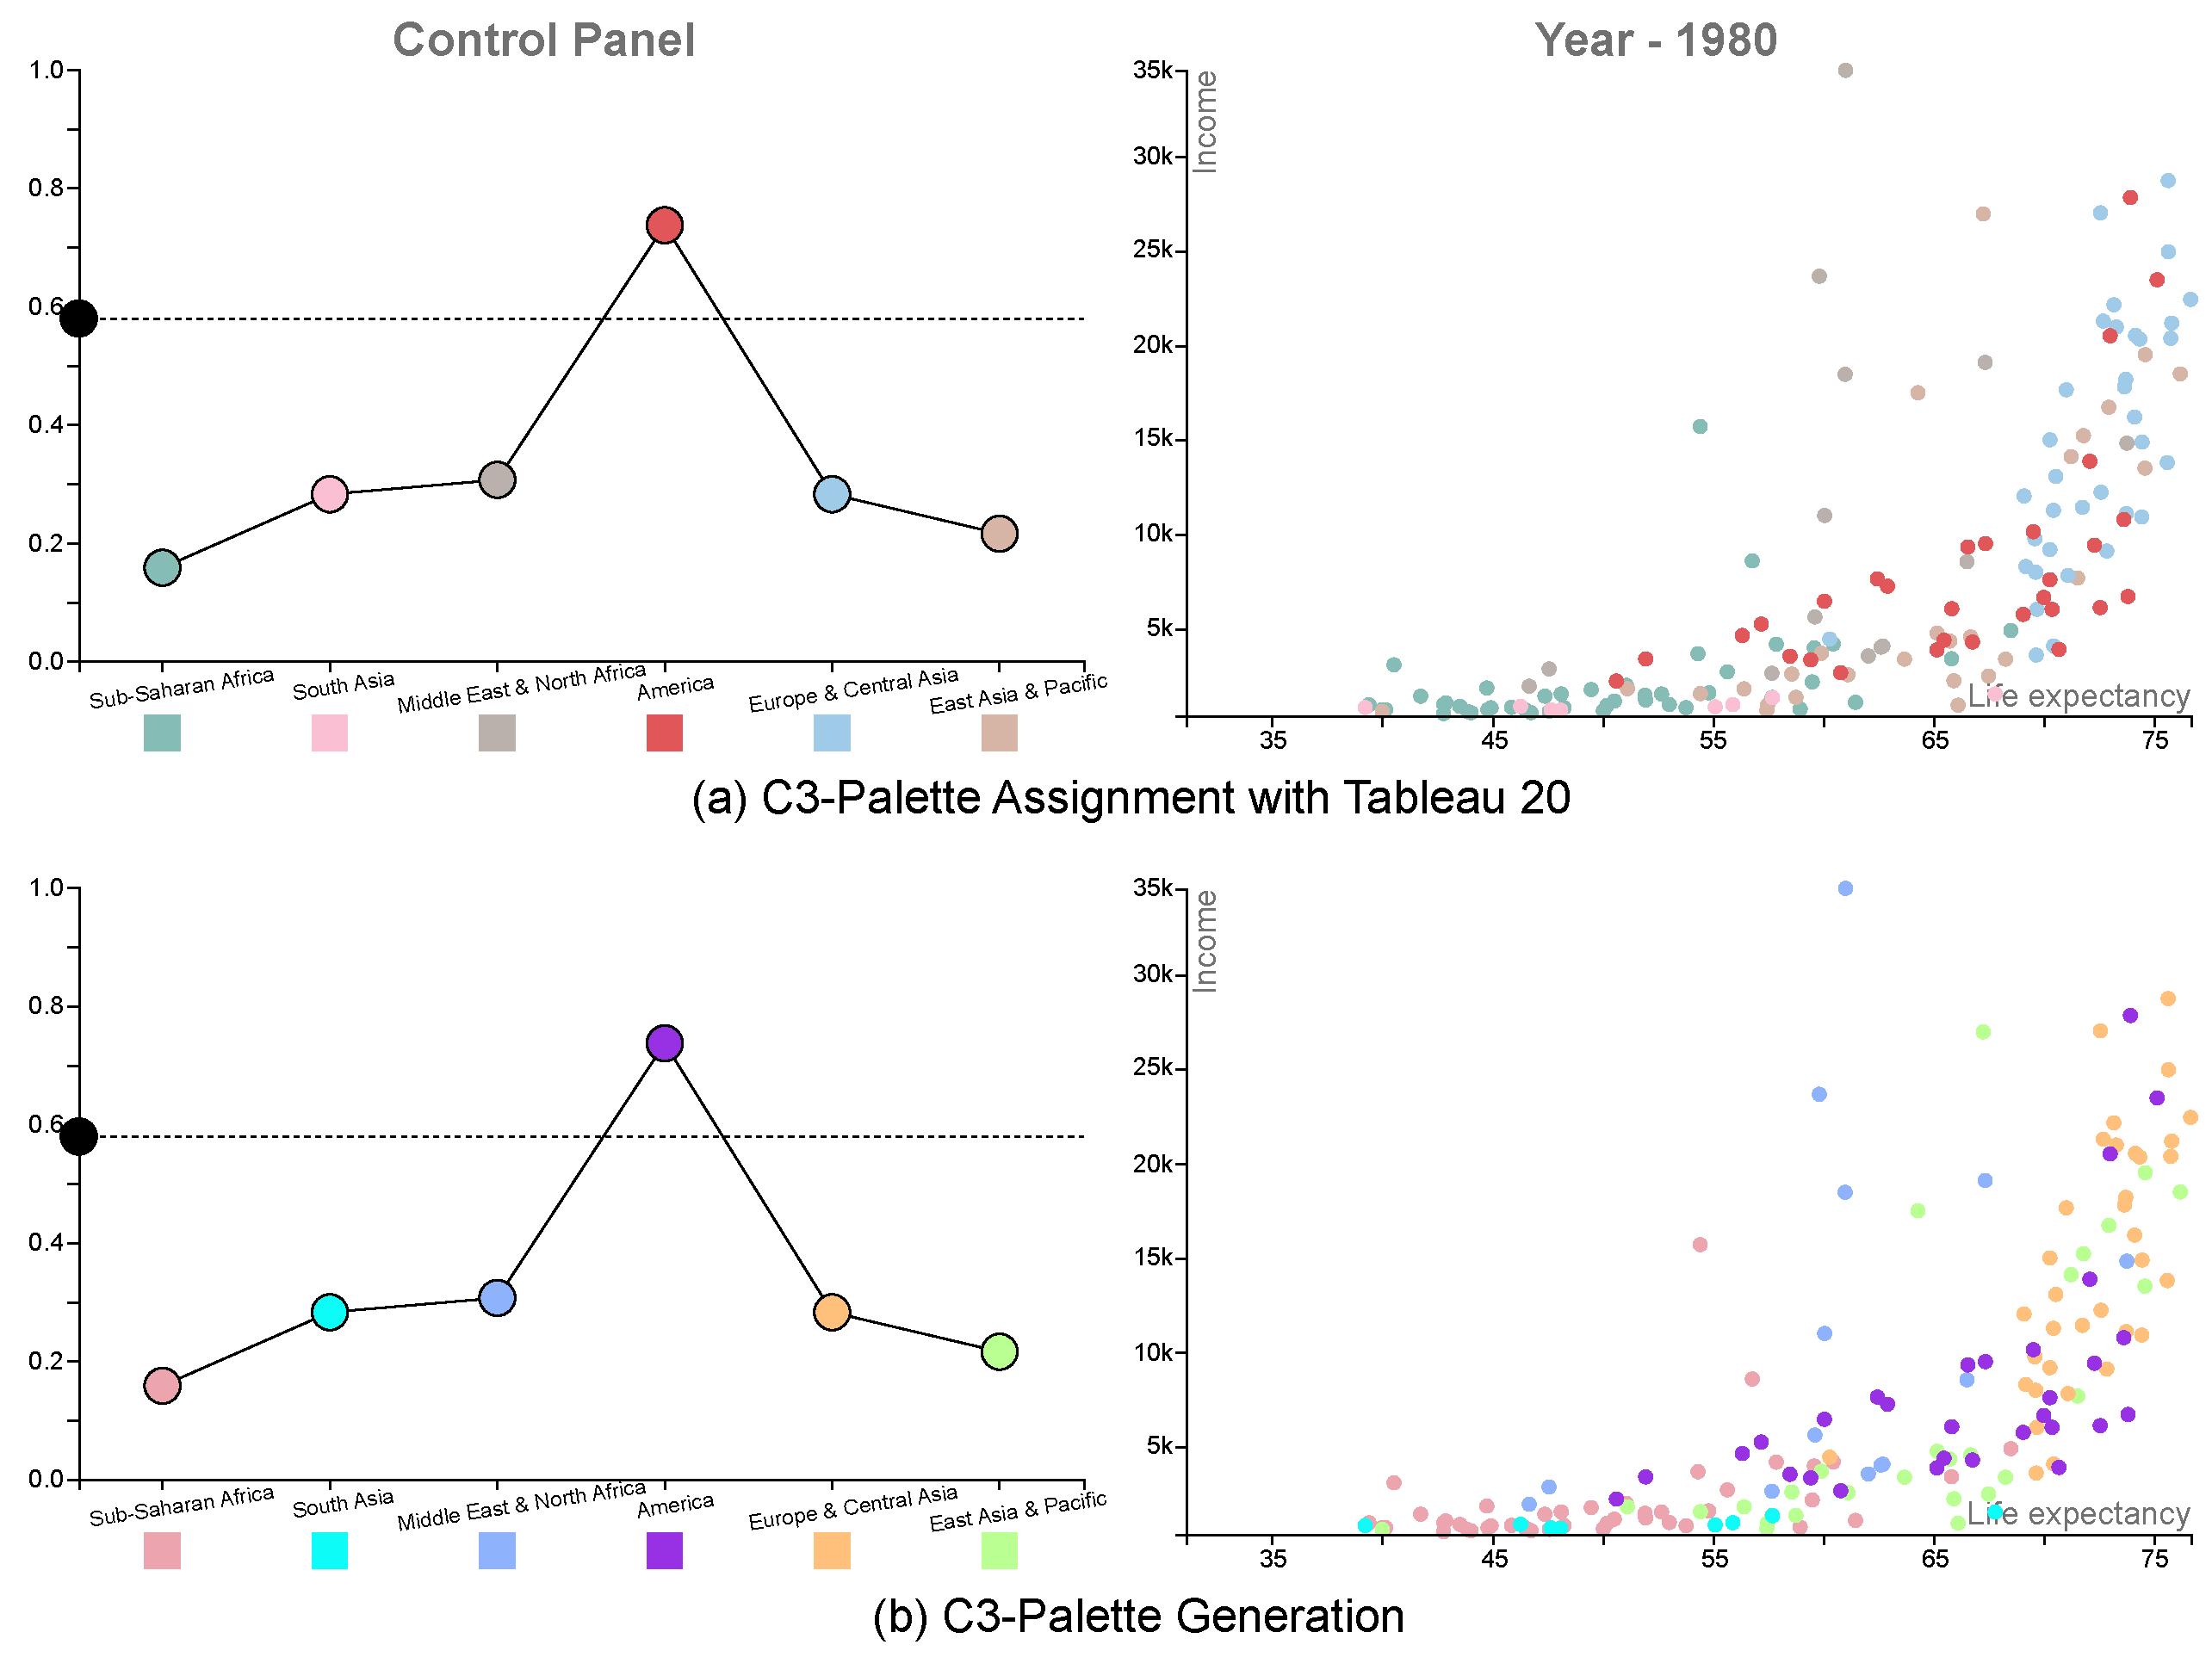
\includegraphics[width=0.8\linewidth]{interaction.pdf}
%\caption{Manually define the class importance in the control panel: (a) Result generated based on given palette; (b) Automatic palette generation.}
%\label{fig:casestudyinteraction}
%\vspace{-4mm}
%\end{figure}
%
%Our system also supports manually class importance adjustment, we illustrate this in Fig.~\ref{fig:casestudyinteraction}. For example, we are interested in \emph{America}, thus we can increase the importance value of the corresponding circle and meanwhile, decrease other classes' importance value until lower than $\kappa$. We show both assignment result for user provided palette and automatic palette generation result. It's obvious that both results highlight the interested class while palette generation method leads to a much better visual separability between different classes.


\CreateLink{huePreserving}{Hue-preserving Palette Generation}
\paragraph{Hue-preserving Palette Generation}.
We also implemented the hue-preserving palette generation which is achieved by adjusting saturation and lightness while maintaining the hue of each color. However, this method cannot produce satisfactory results. As shown in Fig.~\ref{fig:huepreserving} (a), for a single hue value, there exist many different colors. For example, with the same hue (50), we can get black, yellow, grey, brown, etc. Applying this method into our optimization process leads to different colors. Fig.~\ref{fig:huepreserving} (b) shows two examples for different visualization types: the left top scatterplots were generated by default settings, then we maintained the hue of the yellow class in the bottom right and generated new palette, the yellow class changed to grey; this process is similar to line chart, while we maintain the hue of the brown line and finally it changed to grey too. This method is not consistent for user exploration. Hence, we choose color name constraint to maintain consistent color schemes.

\begin{figure*}[h]
\centering
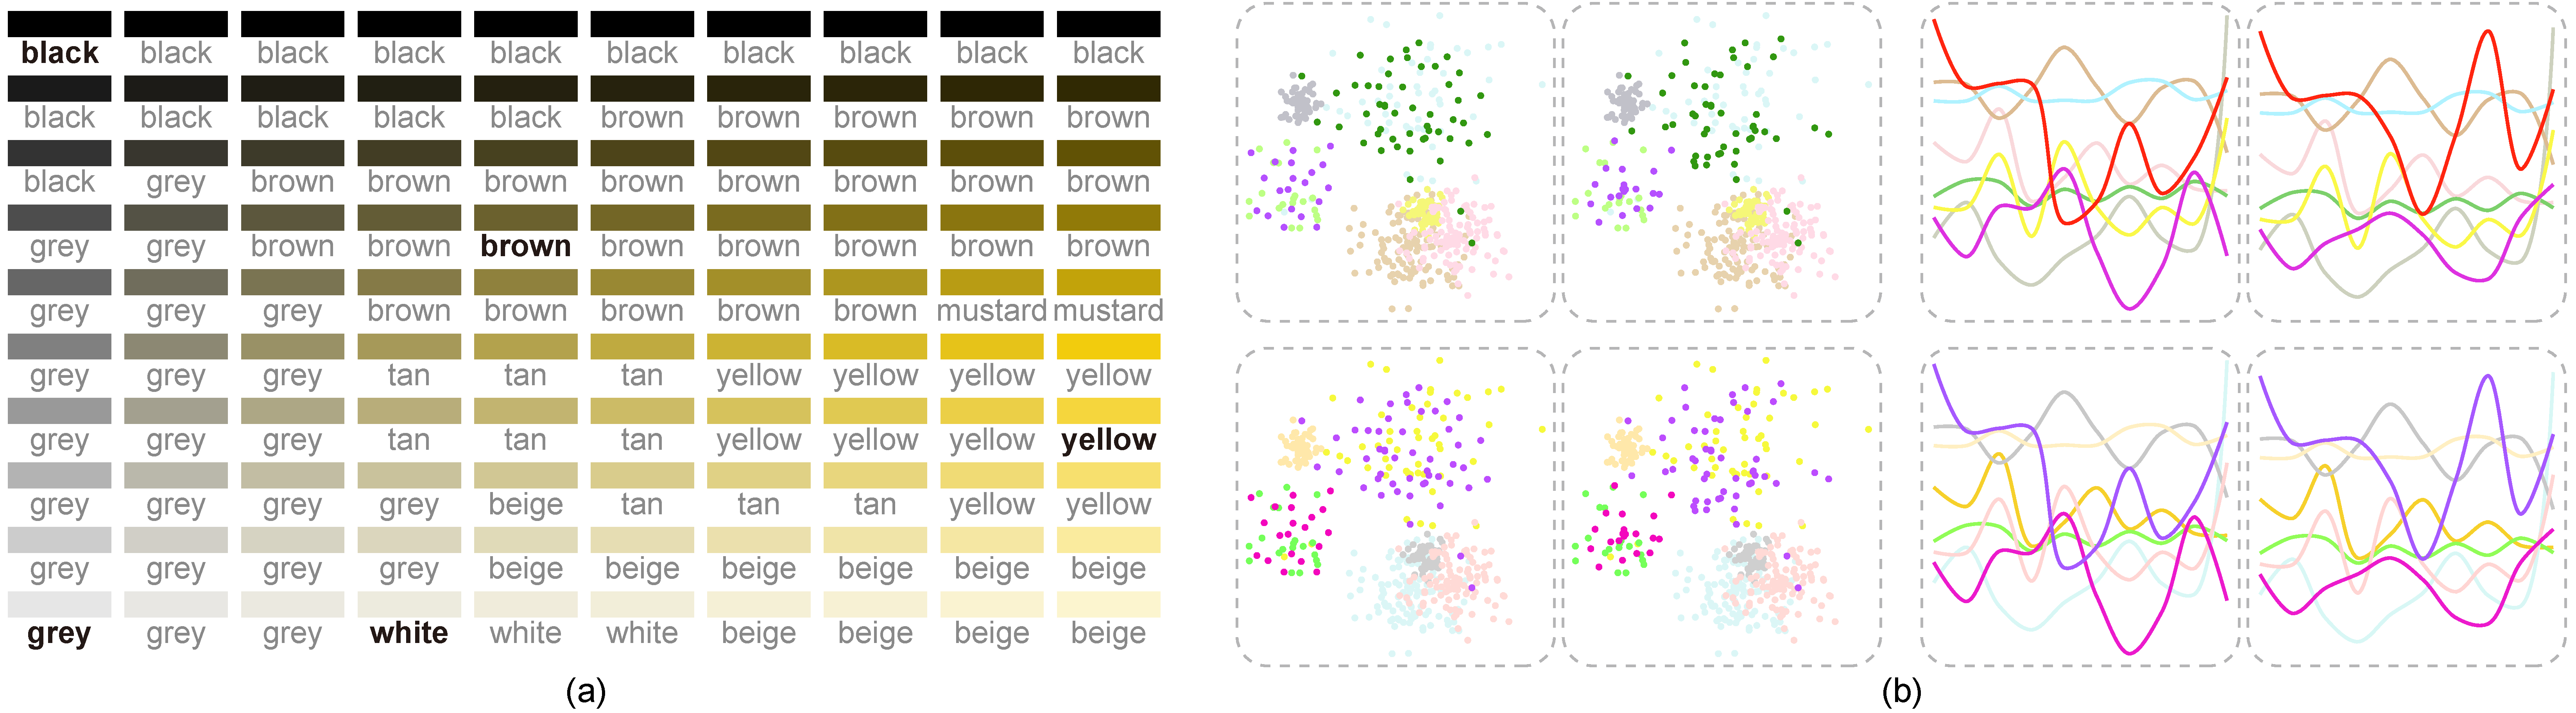
\includegraphics[width=1\linewidth]{hue-preserving.pdf}
\caption{Hue-preserving palette generation. (a) $Hue=50$, quantizing the HSL color space into 100 discrete colors by sampling every 10 units along the saturation and lightness axis starting at the origin, their color name is given below each color; (b) Palette generation results for different visualization types (i.e., scatterplots and line charts): (top) result with default settings; (bottom) hue-preserving results for limiting the hue of the yellow cluster in the top scatterplot and the brown line in the top line chart.}
\vspace*{-5mm}
\label{fig:huepreserving}
\end{figure*}

\CreateLink{colorBlindness}{Palette Generation for Color Vision Deficiency}
\paragraph{Palette Generation for Color Vision Deficiency}.
To help people with color vision deficiency, we allow users to generate palettes that can be used for different types of vision problems, such as protanomaly and deuteranomaly, which result in poor red-green hue discrimination. This is achieved by adopting a color blindness simulator (the source code can be found at GitHub: \url{https://github.com/MaPePeR/jsColorblindSimulator}) and then use our matrix for palette evaluation. Fig.~\ref{fig:blindness} gives an example, where the left two images show the auto-generated results, while the right are simulated results perceived by people with protanomaly. The purple and red classes seen by normal vision will be perceived as dark blue and dark purple by  protanomaly. Our results allow to easily find changes between scatterplots for people with color vision deficiency, which still can be distinguished with normal vision. These preliminary results prove that our method can integrate state-of-the-art color blindness simulation algorithms to generate palettes for color vision deficiency.

\begin{figure}[ht]
\centering
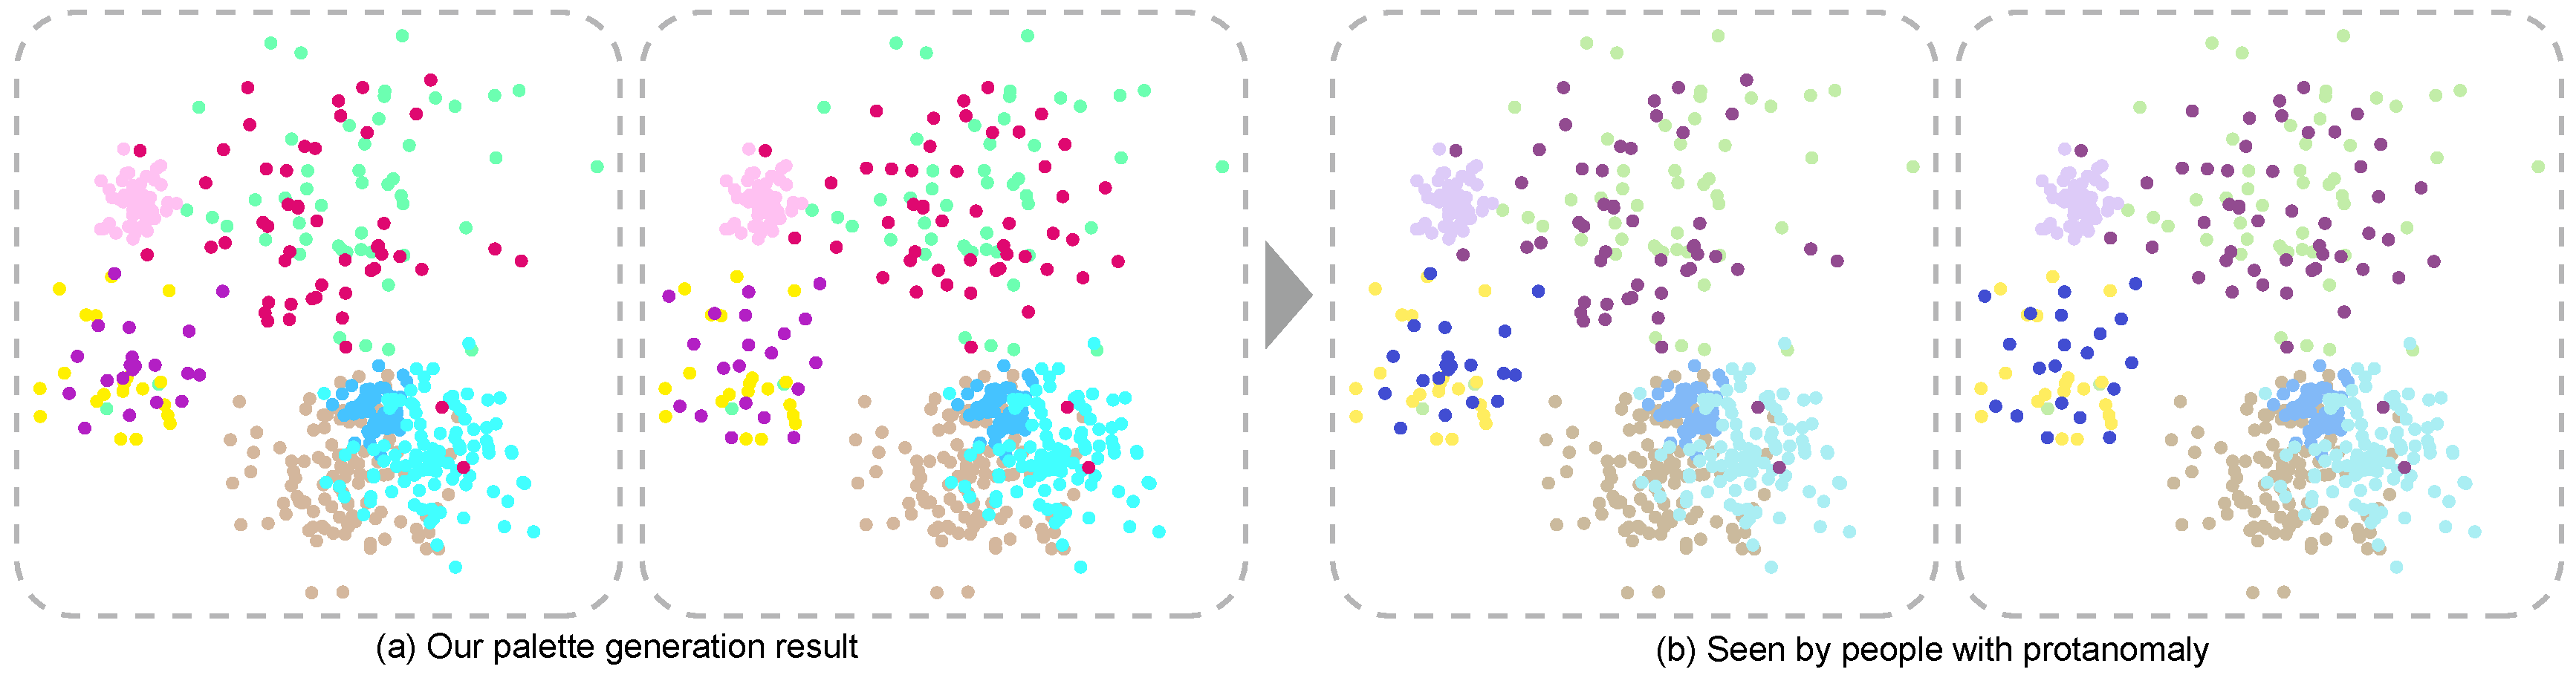
\includegraphics[width=0.96\linewidth]{blindness.pdf}
\caption{Exploring the ability of our system to generate palettes for people with normal vision and also color vision deficiency. (a) The automatically generated palette highlights the two changed classes with a large saliency while maintains a good separability between other classes. (b) Simulated results seen by people with protanomaly. Our results maintain a good performance for both, people with normal vision and color vision deficiency.}
\vspace*{-3mm}
\label{fig:blindness}
\end{figure}

\bibliographystyle{abbrv-doi}
%%use following if all content of bibtex file should be shown
%\nocite{*}
%reference
\bibliography{../cosaliency}

\end{document}
